\documentclass[../notes.tex]{subfiles}

\pagestyle{main}
\renewcommand{\chaptermark}[1]{\markboth{\chaptername\ \thechapter\ (#1)}{}}

\begin{document}




\chapter{???}
\section{Nanomaterials}
\begin{itemize}
    \item \marginnote{1/3:}Contact Dr. Shevchenko at \href{mailto:eshevchenko@anl.gov}{eshevchenko@anl.gov} or \href{mailto:eshevchenko@uchicago.edu}{eshevchenko@uchicago.edu}.
    \item How to make nano.
    \begin{itemize}
        \item Top-down approach: Start with large, end with nano. Includes nanofabrication.
        \item Bottom-up approach: Solution-based approach.
        \begin{itemize}
            \item Scalable and cheap.
            \item Use an inorganic core with a coating.
        \end{itemize}
    \end{itemize}
    \item What nanoparticles look like.
    \begin{itemize}
        \item Differences in size, size distribution, shape, chemical composition, and structures.
        \item Different sizes (like atoms) and different shapes (like bacteria and viri).
    \end{itemize}
    \item Ancient nanoscience.
    \begin{itemize}
        \item The Lycurgus cup.
        \begin{itemize}
            \item A 4th-century Roman glass cage cup.
            \item Currently housed at the British Museum.
            \item Contains $\sim\SI{70}{\nano\meter}$ gold/silver nanoparticles.
            \item When front-lit, it appears green (light is scattered by larger NPs).
            \item When back-lit, it appears red (light is absorbed by NPs).
        \end{itemize}
        \item Hair dye.
        \begin{itemize}
            \item 2000 years ago from Greco-Roman times.
            \item Made of lead oxide (\ce{PbO}), slaked lime (\ce{Ca(OH)2}), and water (\ce{H2O}).
            \item The lead oxide combines with sulfur-rich peptides in the hair to make $\sim\SI{5}{\nano\meter}$ \ce{PbS} NPs.
        \end{itemize}
    \end{itemize}
    \item Applications of nanoparticles: Catalysis.
    \begin{itemize}
        \item Refining of petroleum (transformation of crude oil into gasoline, jet fuel, diesel oil, and fuel oils).
        \item Converter of automobile exhaust (reduction of nitrogen oxides [\ce{NO_x}] to \ce{N2} and \ce{O2}; oxidation of \ce{CO} to \ce{CO2}; oxidation of unburnt hydrocarbons to \ce{CO2 + H2O}).
        \item Hydrogenation of \ce{CO} (synthesis of fuels such as methane or methanol).
        \item Selective oxidation of hydrocarbons (synthetic fibers, plastics, and fine chemicals).
    \end{itemize}
    \item Methods of NP analysis: XRD, TEM, XANES, and XPS.
    \item Applications of nanoparticles: Displays.
    \begin{itemize}
        \item Semiconductor nanoparticles (e.g., solutions of \ce{CdSe} or \ce{InP} nanoparticles) emit different colors.
        \item Sony has announced that it will embed quantum dots in its latest flat-screen TV.
        \item QLEDs can be made out of \ce{CdSe}, \ce{CdS}, \ce{InP} coatings with silica, perovskite (\ce{CsPbX} where $\ce{X}=\ce{Cl},\ce{Br},\ce{I}$), and cesium lead halide salts.
    \end{itemize}
    \item Milestones in the synthesis of nanomaterials (a subjective and incomplete POV).
    \begin{itemize}
        \item Alexei Ekimov (late 1970s-1981, USSR): \ce{CuCl_x} and \ce{CdSe} in molten glass matrix (fluorescence, gradient colors).
        \item Alexander Afros (1982): Theoretical description of size effect.
        \item Louis Brus (1983, Bell Labs, US): \ce{CdS} in solution.
        \item Paul Alivisatos (UChicago) and Moungi Bawendi (MIT).
        \item Moungi Bawendi et al. (1993): Synthesis of monodisperse \ce{CdSe} nanoparticles --- a big one!
        \item Philippe Guyot-Sionnest (1996): Synthesis of core/shell nanoparticles.
        \item Paul Alivisatos (1997 and 2003): Synthesis of nanorods and tetrapods.
        \item Chris Murray and Shouheng Sun (2000): Synthesis of magnetic \ce{FePt} nanoparticles.
        \item Benoit Dubert (2007, France): Synthesis of \ce{CdSe} nanoplates (more stable, emission is polarized and directional).
        \item Maksym Kovalenko (2015): Synthesis of perovskites.
        \item Mostafe El-Sayed, Catherine Murphy, Peidong Yang, and Yunan Xia: Synthesis of \ce{Au} and \ce{Ag} nanoparticles.
    \end{itemize}
    \item Synthesis of nanoparticles.
    \begin{itemize}
        \item The 1993 Bawendi paper.
        \item The innovation was the synthesis of NPs in organic solvents, still widely used today.
    \end{itemize}
    \item LaMer model.
    \begin{itemize}
        \item Precursors under go nucleation, focusing, and "nano"-Ostwald ripening.
        \item Key idea: Separation of nucleation and growth in time.
    \end{itemize}
    \item Nanomaterials: State-of-the-art.
    \begin{itemize}
        \item The chemistry behind QD synthesis is rather simple compared to what is used by organic or coordination chemists, but the field sometimes lacks depth and chemical understanding.
        \item Indeed, only a fraction of reported results have been reproduced, and only a fraction of those have been understood and optimized.
        \item This is a big problem for AI/ML approaches.
        \item During the next 5-10 years, nanomaterials synthesis will progress mostly through systematic mechanistic studies.
    \end{itemize}
    \item Synthesis of nanocrystals without Ostwald Ripening.
    \begin{itemize}
        \item The nanocrystals form and grow during 0.1-1 minute after the start of the reaction.
        \item Annealing at high temperatures (\SIrange{250}{280}{\celsius}) is required to improve crystallinity.
        \item No change in particle size takes place upon the annealing.
        \item Tune particle size with nucleation, since growth proceeds until all monomer is consumed --- fast nucleation leads to many particles, which can only grow so large; slow nucleation leads to a few particles which can grow very large (conservation of end volume).
    \end{itemize}
    \item Synthesis with "artificial molecules."
    \begin{itemize}
        \item Rearrangement, addition, substitution, and elimination.
    \end{itemize}
    \item Hollow nanocrystals: Kirkendal Effect at Nanoscale.
    \begin{itemize}
        \item Uniform spherical cobalt nanocrystals can be synthesized by rapid pyrolysis of cobalt carbonyl in hot solvent.
        \item Hollow nanocrystals form after sulfidation reaction.
    \end{itemize}
    \item Kirkendal effect.
    \begin{figure}[h!]
        \centering
        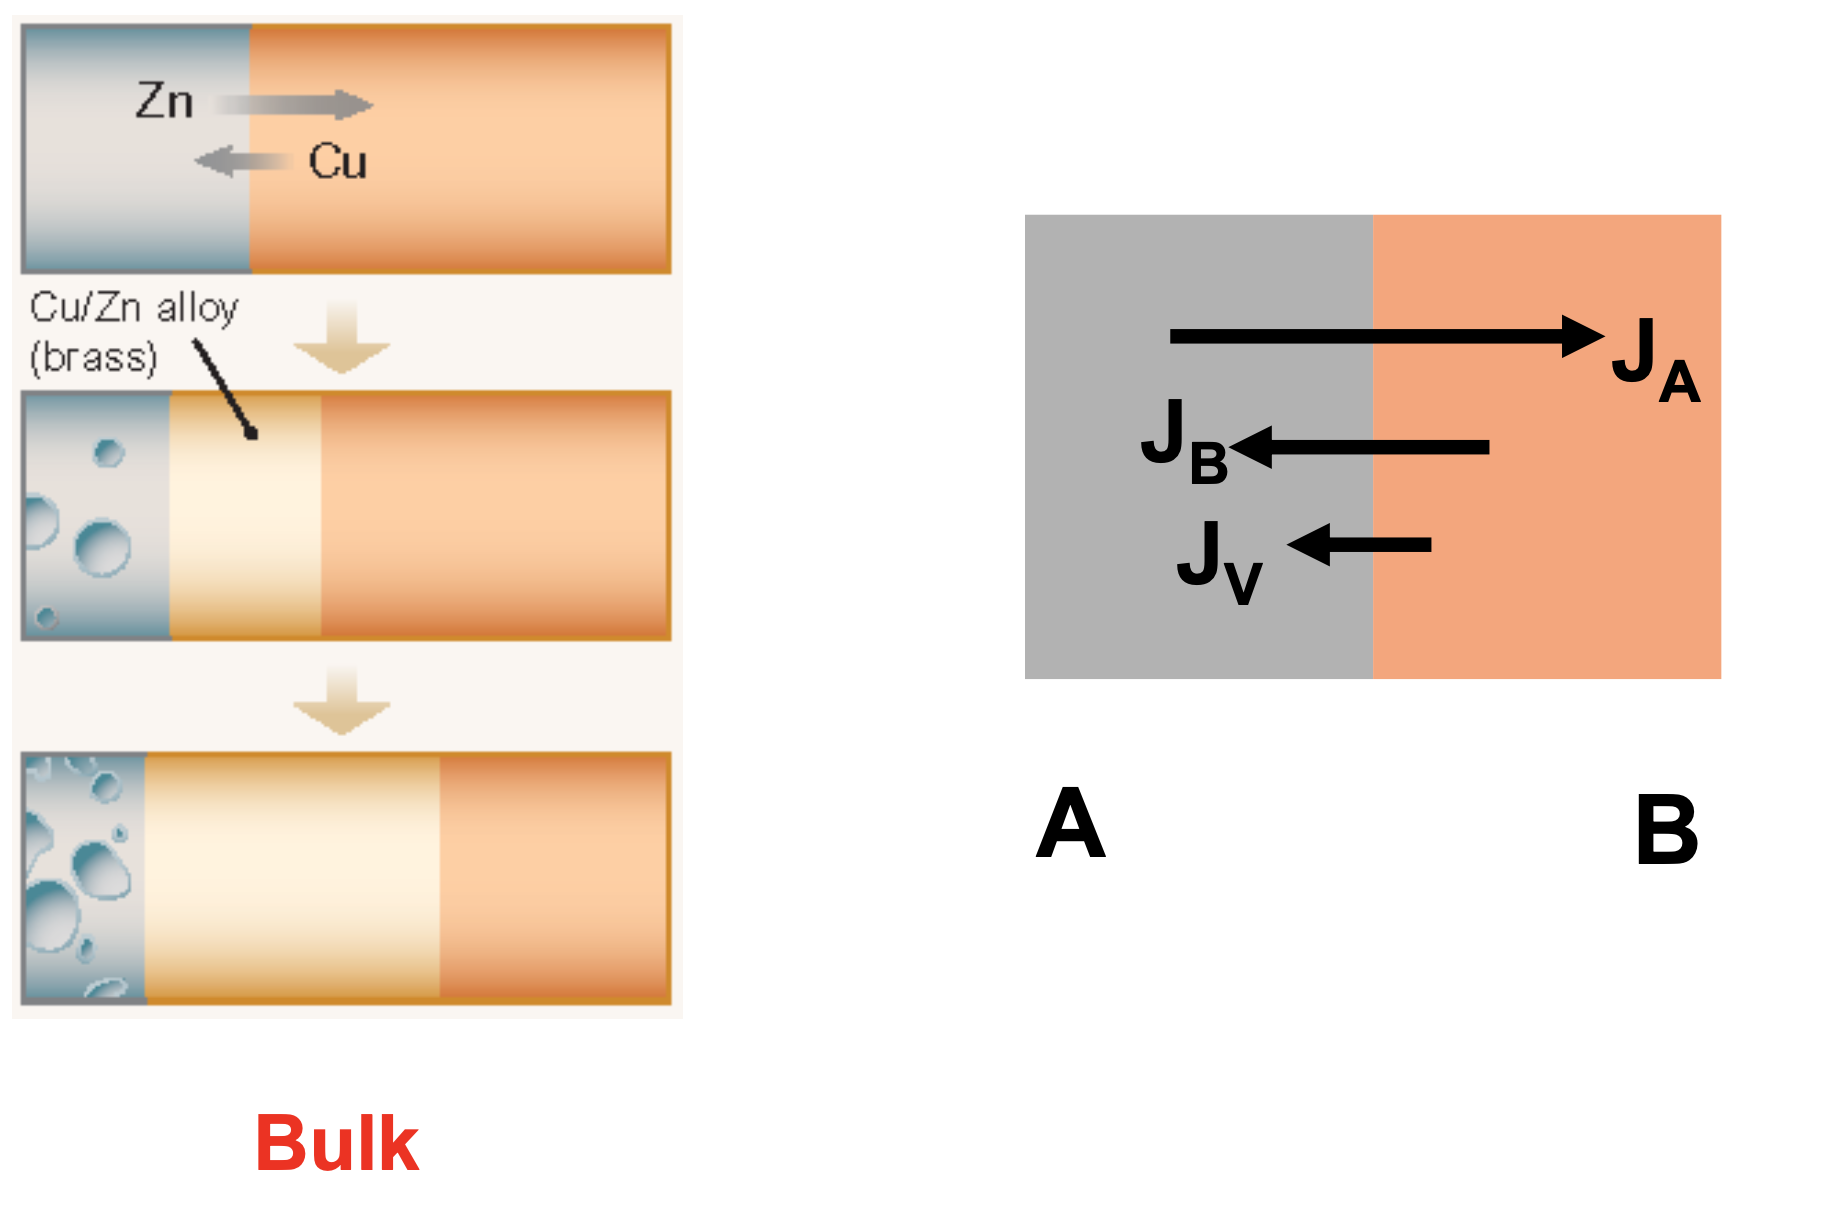
\includegraphics[width=0.43\linewidth]{KirkendalEffect.png}
        \caption{Kirkendal effect.}
        \label{fig:KirkendalEffect}
    \end{figure}
    \begin{itemize}
        \item Occurs when the diffusion rates of two species are different.
        \item When vacancies become supersaturated, they condense into voids in the fast diffusion species side.
        \item The Kirkendall voids result in weak bonding and lead to brittle fracture at the bonding interface.
    \end{itemize}
    \item Top-down approaches for the synthesis of \ce{MoS2}.
    \begin{figure}[h!]
        \centering
        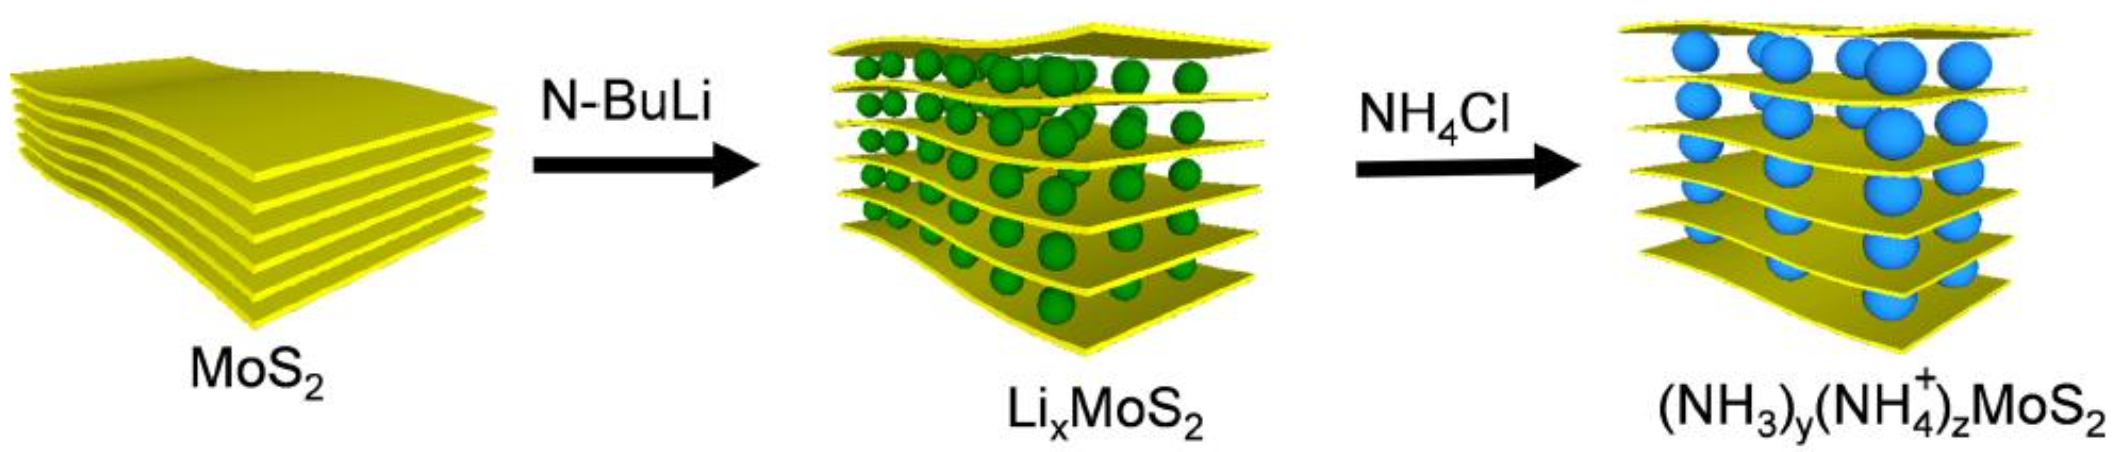
\includegraphics[width=0.6\linewidth]{topDownMoS2.png}
        \caption{Top-down synthesis of \ce{MoS2}.}
        \label{fig:topDownMoS2}
    \end{figure}
    \begin{itemize}
        \item This is the synthesis of interlayer expanded (IE) \ce{MoS2} through chemical intercalation of \ce{Li} and the following exchange with \ce{NH3} and \ce{NH4}.
        \item Each \ce{MoS2} layer is composed of an atomic layer of \ce{Mo} sandwiched between atomic layers of \ce{S} through strong ionic/covalent bonds. Weak van der Waals forces link individual \ce{MoS2} layers with an interlayer spacing of \SI{0.615}{\nano\meter}.
        \item Procedure.
        \begin{itemize}
            \item Electron-donating species, e.g., alkali metals, Lewis bases, and organolithium compounds can intercalate between layers.
            \item Alkali metals can after that be evaporated or react with water.
            \item \textbf{Exfoliation} with ultrasound (mechanical exfoliation).
        \end{itemize}
        \item Useful characterization methods: TEM, XRD, XPS.
    \end{itemize}
    \item \textbf{Exfoliation}: The complete separation of the layers of a material.
    \item Bottom-up approaches for the synthesis of \ce{MoS2}.
    \begin{itemize}
        \item Chemical synthesis of interlayer expanded (IE) \ce{MoS2}.
        \item Chemical Vapor Deposition (CVD).
    \end{itemize}
    \item MXene = 2D metal and surface chemistry.
    \begin{itemize}
        \item Applicatoins to supercapacitors, batteries, conductors, catalysts, and composites.
        \item Most made out of \ce{Ti3AlC2}.
    \end{itemize}
    \item MXenes: Solution processed 2D transition metal carbides and nitrides.
    \begin{itemize}
        \item Scanning electron microscopy (SEM) and HRTEM images shown.
        \item Etching and delamination phases.
    \end{itemize}
    \item MXenes: Variable termination groups.
    \begin{itemize}
        \item Ask in OH??
    \end{itemize}
    \item MXenes are solution processable 2D transition metal carbides and nitrides.
    \begin{itemize}
        \item Lists various experimentally synthesized structures.
    \end{itemize}
    \item What can and cannot be synthesized in solution?
    \begin{itemize}
        \item Current solution synthesis methodology can be applied to materials that crystallize below \SI{400}{\celsius}. Many materials that require higher temperatures to form, e.g., nitrides, carbides, \ce{GaAs}.
        \item Higher temperatures: Gas phase and solid state synthesis, as well as synthesis in molten salts.
    \end{itemize}
    \item Nanocrystals in molten salts.
    \begin{itemize}
        \item QDs are synthesized at high T in molten salts.
        \item There is typically a postpreparative treatment phase still in molten salts.
    \end{itemize}
    \item Nanoparticles as building blocks to make new materials.
    \begin{itemize}
        \item The idea behind nanoparticles is encapsulated by the synthesis of \ce{NaCl} from \ce{Na${}^\circ$} and \ce{Cl2${}^\circ$}: Two substances with certain properties combine to form a new material with very different properties.
        \item Assembly of atoms leads to new materials and new properties!
    \end{itemize}
    \item Self-assembly of nanoparticles.
    \begin{itemize}
        \item Can be multilayered (up to five).
    \end{itemize}
    \item Crystals of nanocrystals.
    \begin{itemize}
        \item Example: 3D crystals ($\sim\SI{30}{\micro\meter}$) have been assembled from \SI{3.3}{\nano\meter} \ce{CdSe} nanocrystals.
        \item Example: 3D crystals ($\sim\SI{10}{\micro\meter}$) have been assembled from \SI{6}{\nano\meter} \ce{CoPt3} nanocrystals.
        \item More conventional example: Crystals of quartz (made by atoms).
    \end{itemize}
    \item Binary nanoparticle superlattices.
    \begin{itemize}
        \item Natural opal vs. synthetic opals (very similar appearance and properties).
        \item Formation of binary superlattices depends on the ratio of nanoparticle radii ($\gamma$), the concentration of nanoparticles, the size distribution of nanoparticles, the nature of the capping ligand, and the substrate.
        \item Evaporating colloidal solutions of binary nanoparticle mixtures at \SI{45}{\celsius} leads to the formation of binary nanoparticle superlattices.
    \end{itemize}
    \item Periodic table of nanocrystals.
    \begin{itemize}
        \item Different types of unit cells listed.
        \item Examples include \ce{AlB2}, \ce{MgZn2}, \ce{Cu3Au}, \ce{Fe4C}, \ce{CaCu5}, and \ce{CaB6}.
    \end{itemize}
    \item Directing of self-assembly of nanocrystals.
    \begin{itemize}
        \item Various additives can be mixed in.
    \end{itemize}
    \item Metal organic frameworks (MOFs).
    \begin{itemize}
        \item MOFs (also called porous coordination polymers or PCPs) are two- or three-dimensional porous crystalline materials with infinite lattices synthesized from secondary building units (SBUs) --- metal cations, salts, or clusters --- and polydentate organic ligands with coordination type connections.
        \item Common SBUs pictured.
        \item From single-metal nodes to SBUs: More than 20,000 MOF structures have been reported so far.
        \item Characterization methods: TEM, SEM, XRD, XANES, XPS, and electron paramagnetic resonance (EPR).
    \end{itemize}
    \item Summary.
    \begin{itemize}
        \item Structural information (XRD, ED).
        \item Compositional information (XRD, ED, energy dispersive X-ray analysis [EDX], and X-ray fluorescence [XRF]).
        \item Size and morphology of materials (TEM, SEM, and XRD).
        \item Redox states of bulk and surface (XANES, XPS).
        \item Important variables: Quality of synthesized materials, stability of materials during processes, and structure-property correlations.
    \end{itemize}
\end{itemize}




\end{document}